\documentclass[UTF8]{ctexart}
\usepackage{graphicx}
\usepackage{multirow}
\usepackage{booktabs}
\usepackage{indentfirst}
\setlength{\parindent}{2em}
\usepackage{color}
\definecolor{lbcolor}{rgb}{0.9,0.9,0.9}
\usepackage{listings}
\lstset{backgroundcolor=\color{lbcolor}}
\lstset{keywordstyle=\color[rgb]{0,0,1}}
\lstset{commentstyle=\color[rgb]{0.133,0.545,0.133}}
\lstset{stringstyle=\color[rgb]{0.627,0.126,0.941}}
\lstset{language=Matlab}
\lstset{numbers=left}
\lstset{breaklines=true}
\author{何舜成}
\title{系统工程导论第七章作业}
\begin{document}
\maketitle
\section{计算结果}
选择k=2,最终可得如下分类结果:(五角星为每一类的中心点)\par
\begin{figure}[tbp]
  \centering
  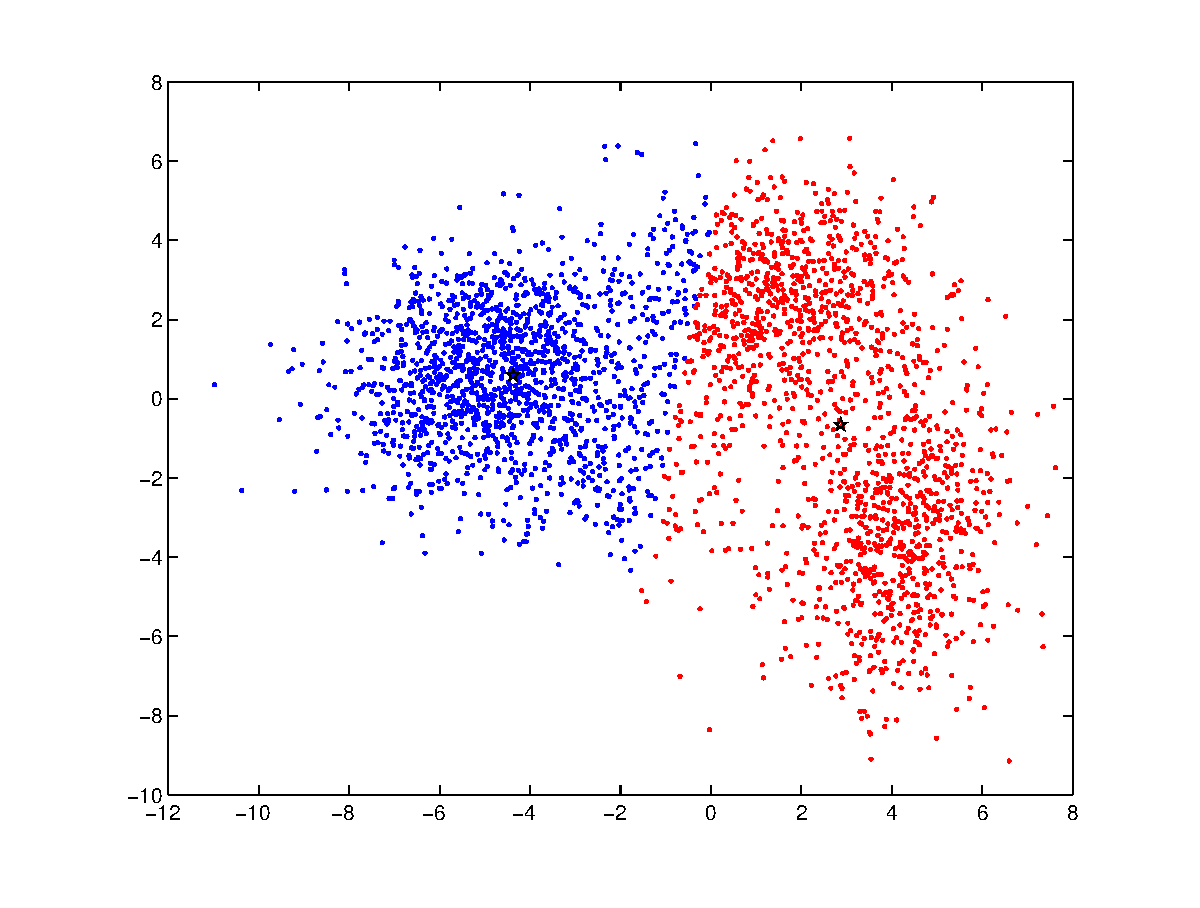
\includegraphics[width=1.05\textwidth]{kmeans2.eps}
\end{figure}
\par
其中计算过程迭代8次,用时1.0486s\par
选择k=3:\par
\begin{figure}[tbp]
  \centering
  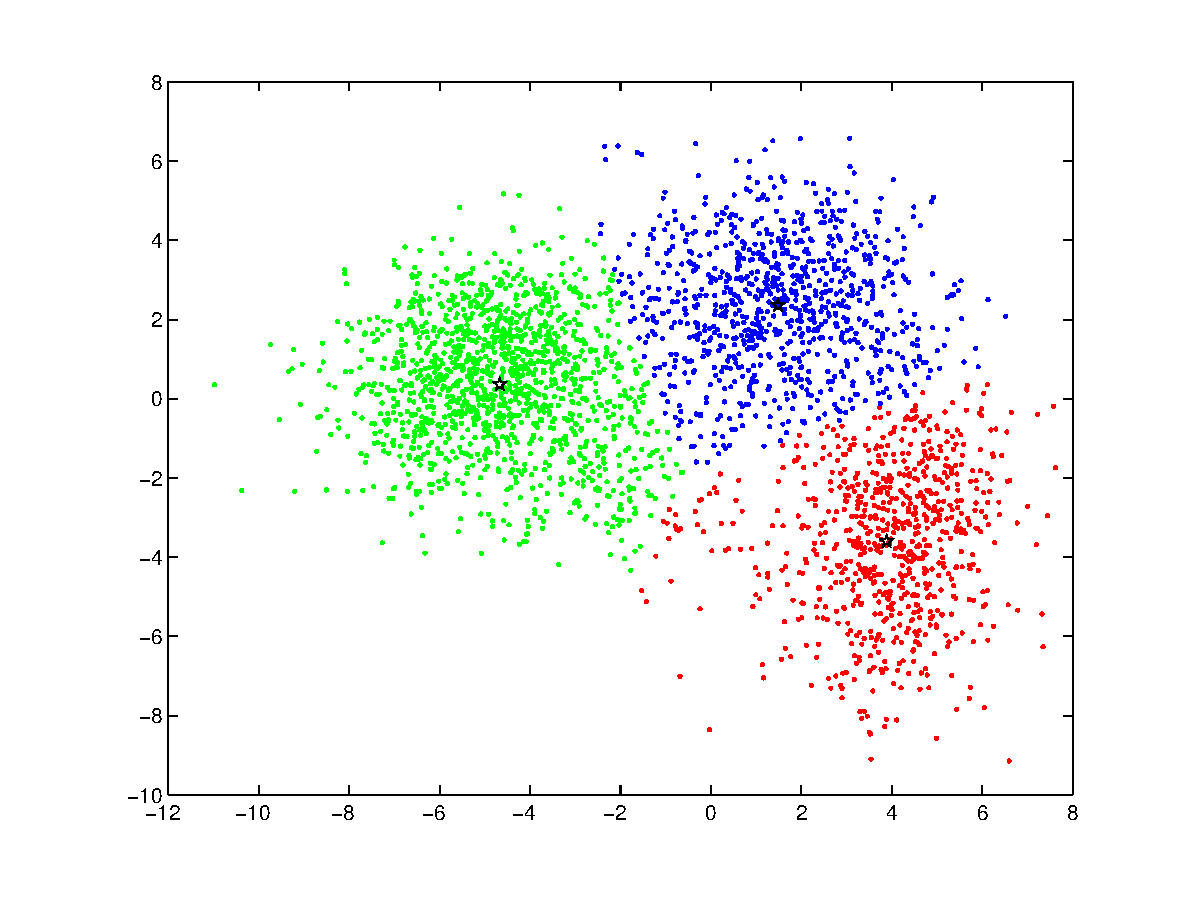
\includegraphics[width=1.05\textwidth]{kmeans3.eps}
\end{figure}
\par
计算过程迭代5次,用时0.7576s\par
选择k=4:\par
\begin{figure}[tbp]
  \centering
  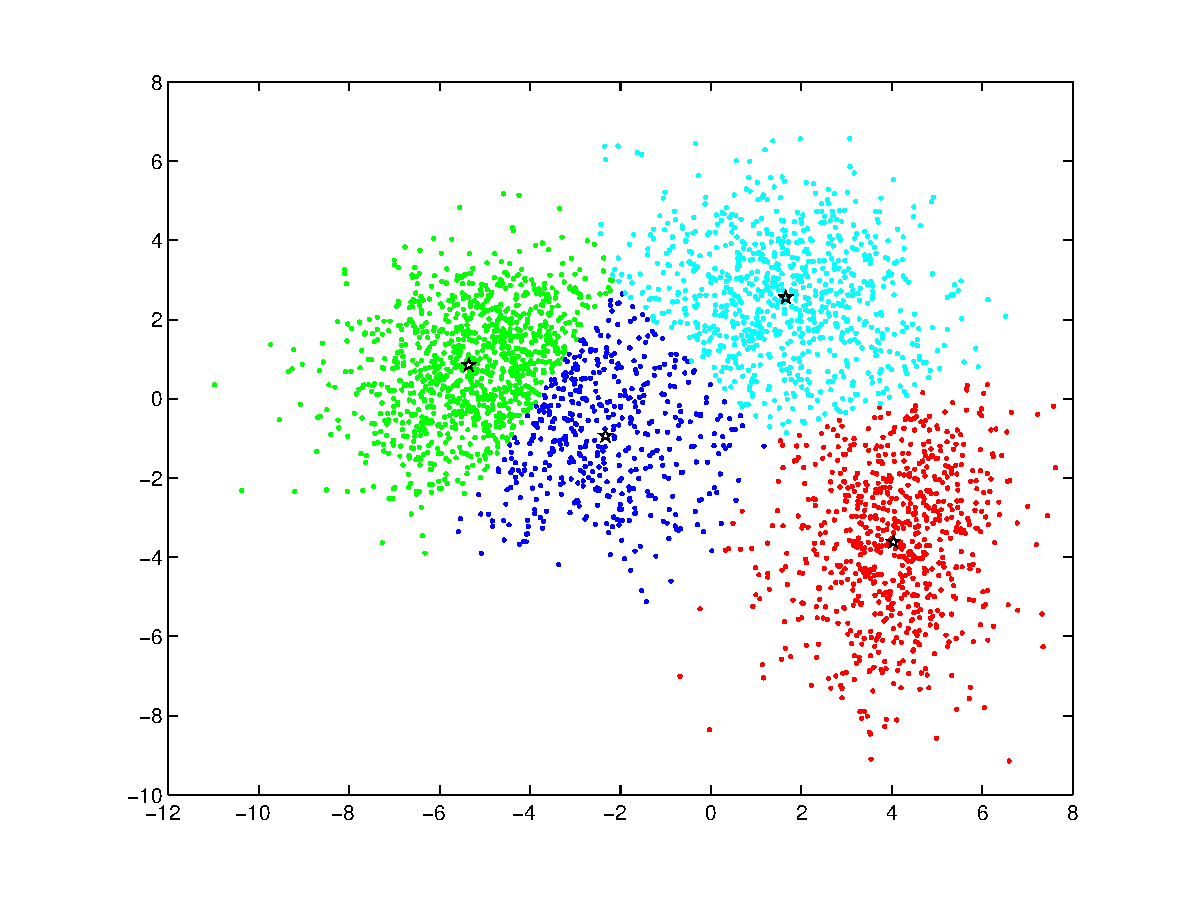
\includegraphics[width=1.05\textwidth]{kmeans4.eps}
\end{figure}
\par
计算过程迭代12次,用时1.8084s\par
选择k=5:\par
\begin{figure}[tbp]
  \centering
  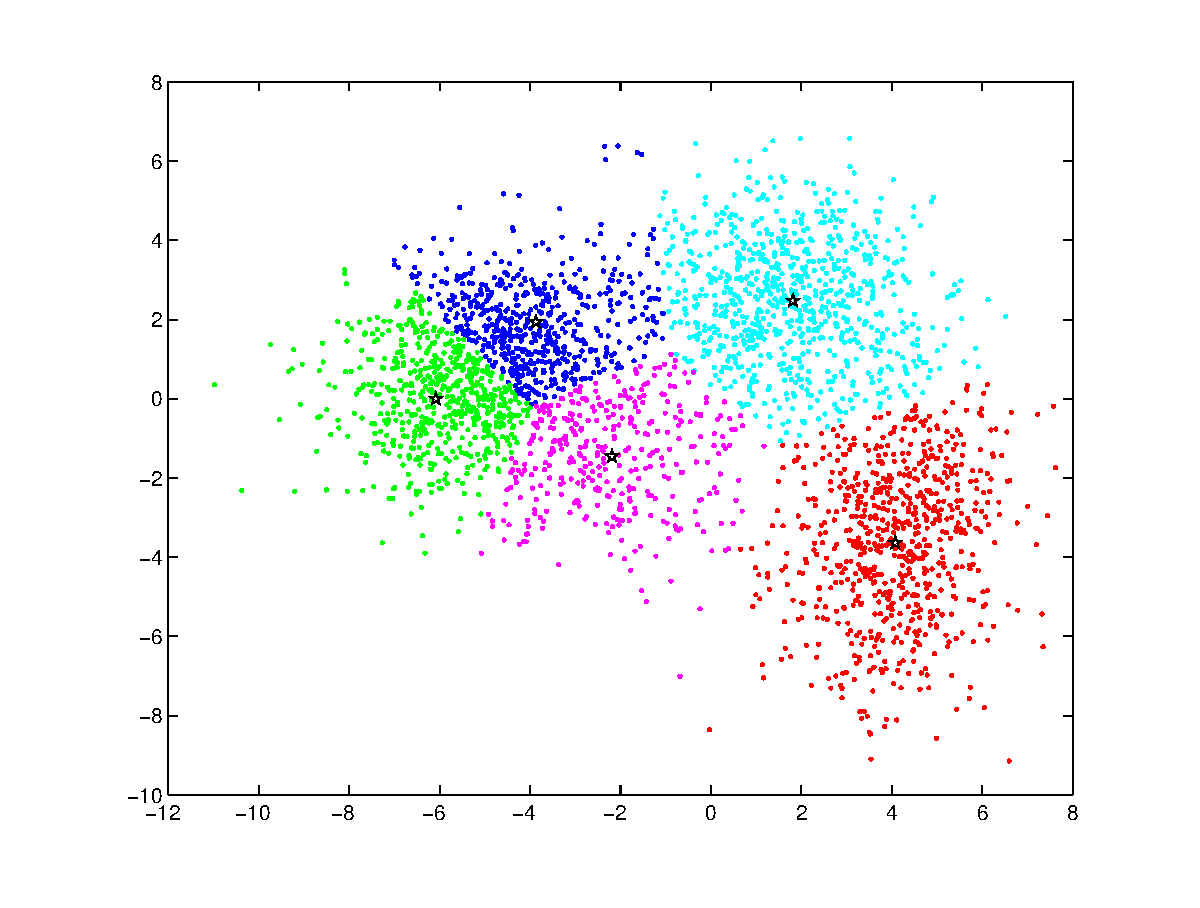
\includegraphics[width=1.05\textwidth]{kmeans5.eps}
\end{figure}
\par
计算过程迭代16次,用时2.4336s\par
选择k=3:\par
\begin{figure}[h]
  \centering
  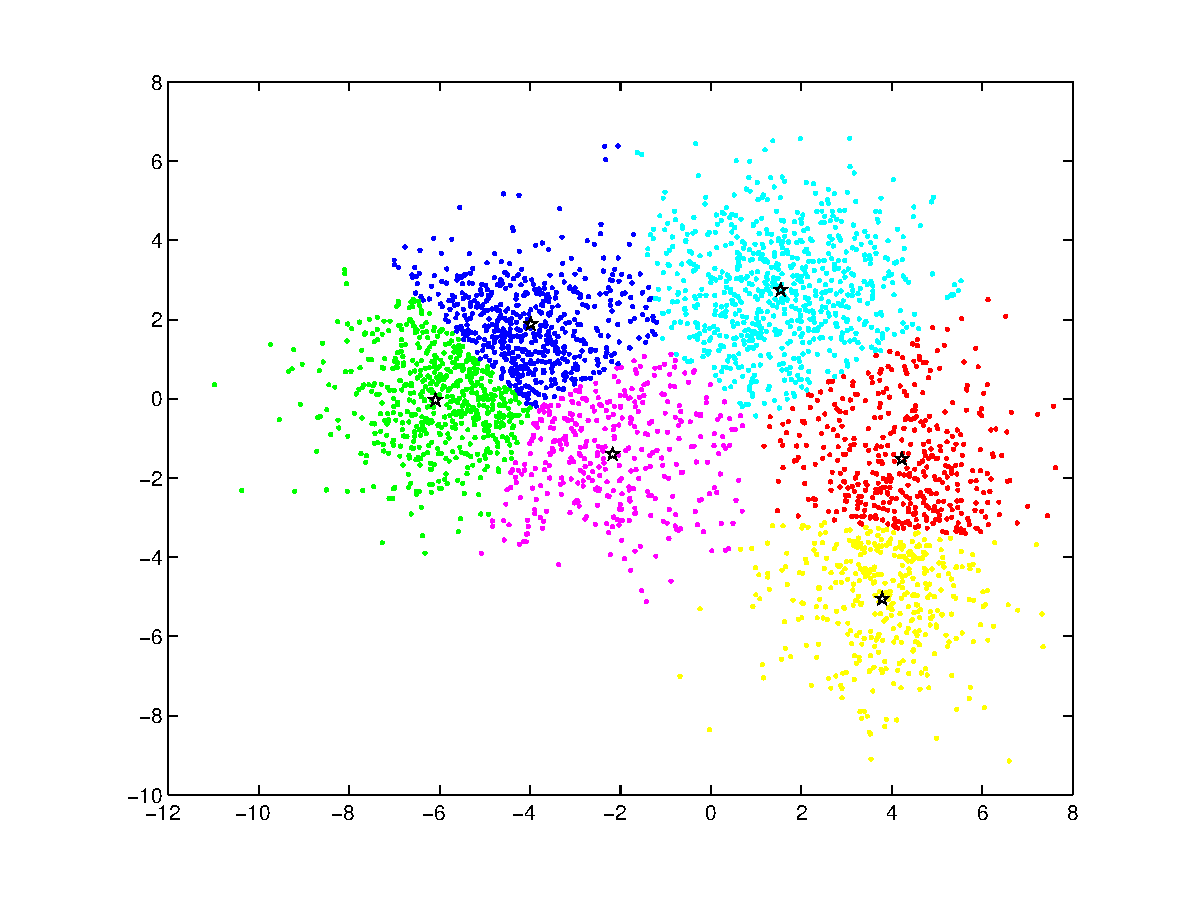
\includegraphics[width=1.05\textwidth]{kmeans6.eps}
\end{figure}
\par
计算过程迭代65次,用时9.6139s\par

\section{具体实现}
Matlab代码(.m文件)如下所示:\par
\begin{lstlisting}
function label=kmeans_clustering(data,num)
k = num;
dsize = size(data);
N = dsize(1);
m = dsize(2);
center = data(N-k+1:N,:);
rho = inf;
label = zeros(N,1);
iter = 0;
while(0 < 1)
    newrho = 0;
    for p=1:N
        dist = inf;
        label(p) = 0;
        for q=1:k
            if norm(center(q,:)-data(p,:))<dist
                dist = norm(center(q,:)-data(p,:));
                label(p) = q;
            end
        end
        newrho = newrho + dot(data(p,:)-center(label(p),:),data(p,:)-center(label(p),:));
    end
    if abs(rho-newrho)<1e-4
        break;
    end
    rho = newrho;
    center = zeros(k,m);
    total = zeros(k,1);
    for p=1:N
        total(label(p)) = total(label(p)) + 1;
        center(label(p),:) = center(label(p),:) + data(p,:);
    end
    for q=1:k
        center(q,:) = center(q,:)./total(q);
    end
    iter = iter + 1;
    fprintf('iter = %d, rho = %f\n',iter,rho);
end
\end{lstlisting}
\end{document}